\documentclass[12pt]{article}

\usepackage[utf8]{inputenc}
\usepackage[T2A]{fontenc}
\usepackage[english,russian]{babel}
\usepackage{paratype}
\usepackage{verbatim}
\usepackage{caption}
\captionsetup[figure]{skip=1pt}
\usepackage{microtype}
\usepackage[style=numeric, sorting=none]{biblatex}
\addbibresource{refs.bib}
\usepackage{amssymb,amsmath,amsthm,amsfonts}
\usepackage{gensymb}
\usepackage{booktabs}
\usepackage{geometry}
\usepackage{indentfirst}
\usepackage{pdfpages}
\usepackage{graphicx}
\graphicspath{ {../vis/} }
\usepackage[table,xcdraw]{xcolor}
\usepackage{hyperref}
\hypersetup{
    colorlinks=true,
    linkcolor=blue,
    filecolor=blue,      
    urlcolor=blue,
}

\usepackage{tocloft}
\renewcommand{\cftsecleader}{\cftdotfill{\cftdotsep}}

% \usepackage{fancyhdr}
\geometry{a4paper, textwidth=16cm, textheight=24cm}
\usepackage[italic]{mathastext}

\makeatletter
\renewcommand{\@seccntformat}[1]{}
\makeatother

\begin{document}
\begin{titlepage}
\begin{center}
    Московский государственный университет имени М. В. Ломоносова

    \bigskip
    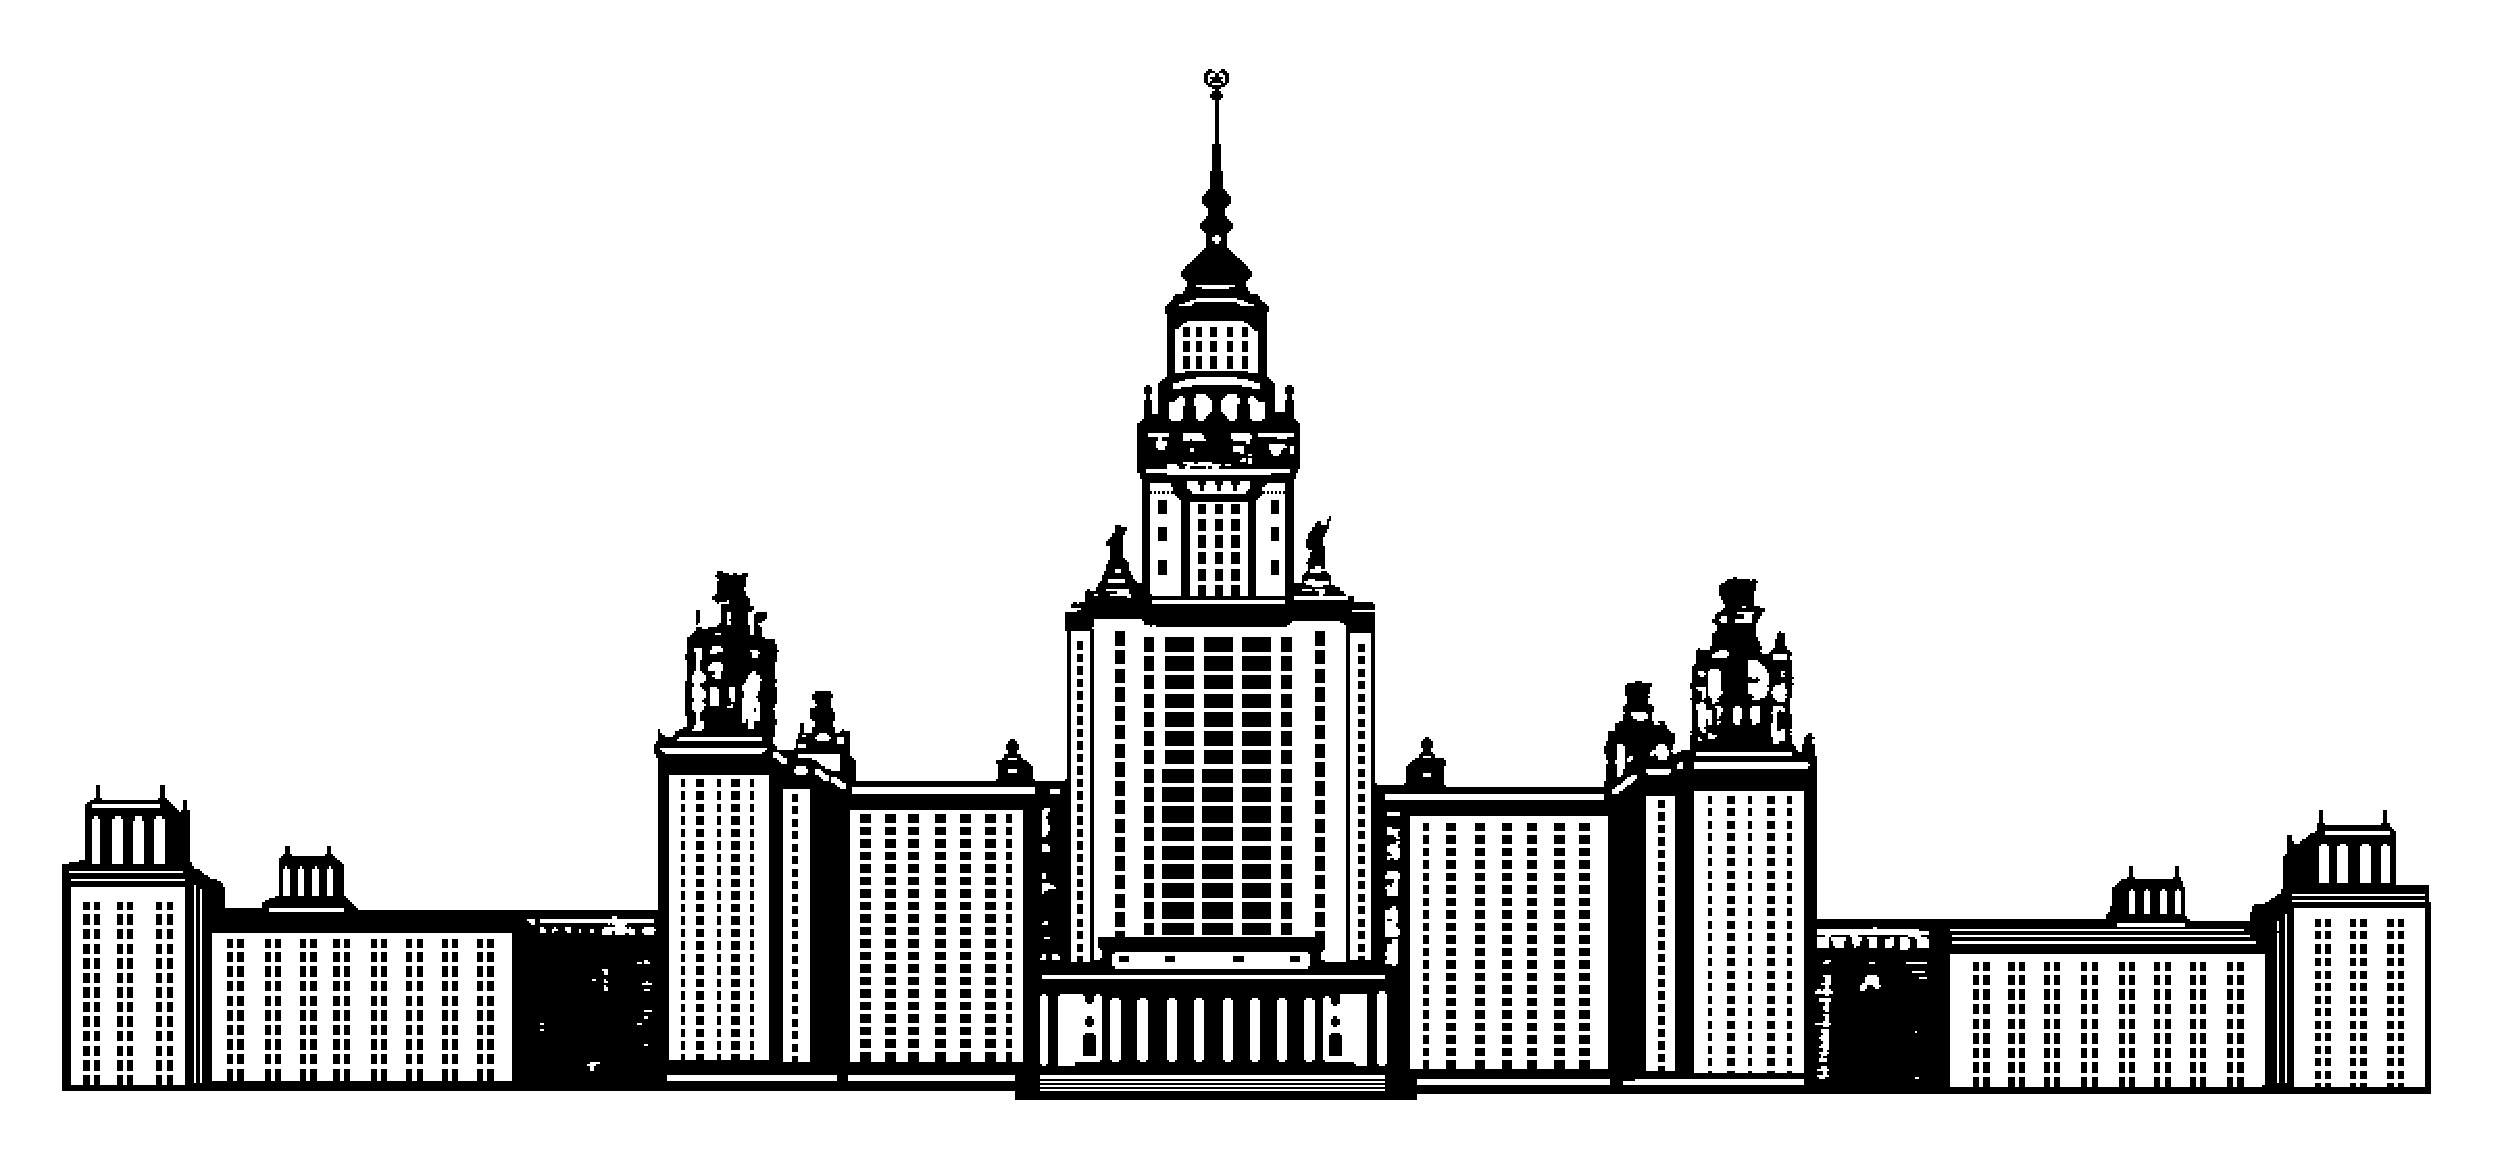
\includegraphics[width=50mm]{msu.eps}

    \bigskip
    Факультет Вычислительной Математики и Кибернетики\\
    Кафедра Математических Методов Прогнозирования\\[10mm]

    \textsf{\large\bfseries
        ОТЧЁТ ПО ЗАДАНИЮ №1\\[10mm]
        <<Метрические алгоритмы классификации>>\\
    }\\[10mm]

    \begin{flushright}
        \parbox{0.5\textwidth}{
        	Выполнил:\\
        	студент 3 курса 317 группы \\
        	\emph{Суглобов Кирилл Алексеевич}\\[5mm]
        }
    \end{flushright}

    \vspace{\fill}
    Москва, 2021
\end{center}
\end{titlepage}
\tableofcontents

\section{Введение}
В задании требовалось написать реализации метода ближайших соседей и кросс-валидации, ознакомиться с метрическими алгоритмами классификации и методами работы с изображениями. В отчёте описывается ход экспериментов, которые выполнялись с помощью написанных на Python модулей, на датасете MNIST, и их результаты.
Далее, если не оговорено иного, предполагается следующее разбиение датасета:
\begin{itemize}
  \item Обучающая выборка: первые 60~000 объектов
  \item Тестовая выборка: последние 10~000 объектов
\end{itemize}

\section{Эксперимент №1: самый быстрый алгоритм}
В эксперименте №1 требуется сравнить время работы алгоритмов написанного kNN-классификатора на примере поиска 5-ти ближайших соседей для каждого объекта тестовой выборки в зависимости от количества признаков (от размерности признакового пространства). Тестовая выборка берётся блоками по 1000 объектов: это используется только в алгоритмах, которые строят в памяти матрицу попарных расстояний (переборные алгоритмы \verb|my_own|, \verb|brute|). 

\begin{figure}[!h]
    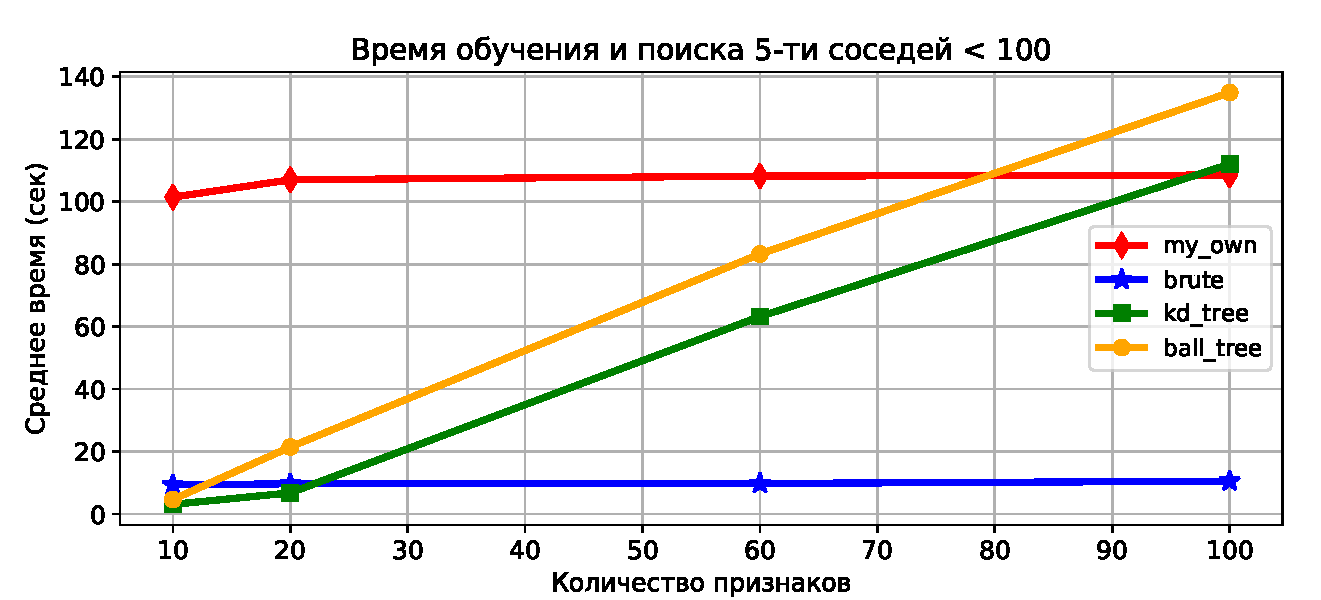
\includegraphics[width=\textwidth]{1_times-1.pdf}
    \caption{}
    \label{fig:1_times-1}
\end{figure}

На \autoref{fig:1_times-1} изображён график для малого числа признаков. Видно, что \verb|tree|-стратегии (деревья) имеют преимущество только в случае малого числа признаков: здесь до 10 признаков преимущество у \verb|kd_tree| и \verb|ball_tree|, до 20 признаков преимущество сохраняется для \verb|kd_tree|. На малом числе признаков \verb|ball_tree| медленнее \verb|kd_tree|. После примерно 20-ти (22-х) признаков преимущество по скорости работы берёт на себя \verb|brute|-стратегия. На время работы переборных алгоритмов количество признаков почти не влияет. Теперь рассмотрим ситуацию, когда > 100 признаков.

\begin{figure}[!h]
    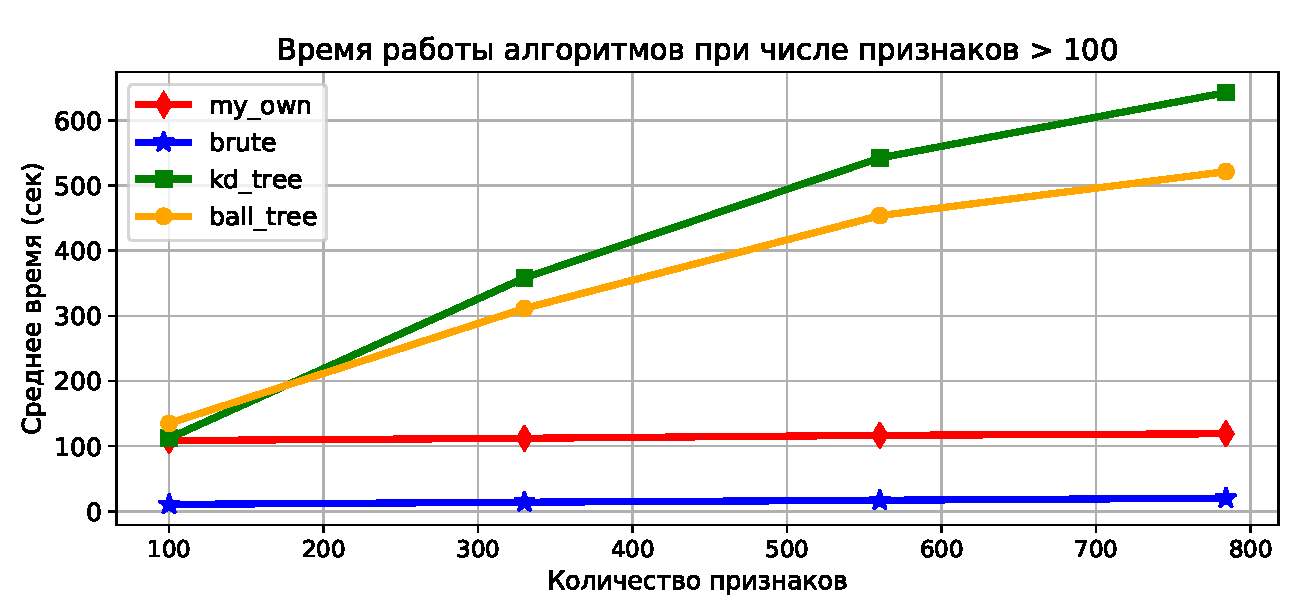
\includegraphics[width=\textwidth]{1_times-2.pdf}
    \caption{}
    \label{fig:1_times-2}
\end{figure}

На \hyperref[fig:1_times-2]{рис. 2} изображён график для большого числа признаков (> 100). Видно, что время работы \verb|tree|-стратегий сильно быстро растёт с ростом количества признаков. Это идёт вразрез с логарифмической асимптотикой работы этих стратегий, которая верна для случаев сбалансированных деревьев с «хорошим» (равномерным) распределением признаков в признаковом пространстве. Но здесь размерность признакового пространства растёт, что вызывает «проклятие размерности»: 60~000 объектов с 784-мя признаками у каждого недостаточно для равномерного покрытия этого пространства.

Рост количества признаков до 784 по-прежнему, как и в случае малого количества признаков, почти не влияет на время работы переборных алгоритмов: \verb|brute| и \verb|my_own|.

Далее будет использоваться алгоритм \verb|brute|, как самый быстрый, и алгоритм \verb|my_own|, по необходимости. \verb|tree|-стратегии показали, что они неэфффективны при размерностях нашей задачи.

\section{Эксперименты №2 и №3: выбор лучшей метрики,\\добавление весов}
В эксперименте №2 требуется оценить по кросс-валидации с 3 фолдами качество, т.е \emph{accuracy} (долю правильно предсказанных ответов) и время
работы алгоритма поиска k ближайших соседей в зависимости от следующих факторов:
\begin{enumerate} 
    \begin{enumerate} 
        \item k от 1 до 10 (только влияние на качество).
        \item Используется евклидова или косинусная метрика.
    \end{enumerate} 
\end{enumerate}

В эксперименте №3 требуется сравнить взвешенный метод $k$ ближайших соседей с методом без весов при тех же фолдах и параметрах. Во взвешенном методе голос объекта равен не $w = 1$ (случай без весов), а $w = \frac{1}{d+10^{-5}}$, где $d$~--- расстояние (по одной из метрик в признаковом пространстве) между объектом и рассматриваемым соседом.

Кроме того, требуется измерить время на кросс-валидации и подобрать оптимальное для качества значение $k$~--- количество ближайших соседей.

В эксперименте использовался алгоритм \verb|brute| с метриками \emph{euclidean} и \emph{cosine}, с весами и без весов.

\begin{figure}[!h]
    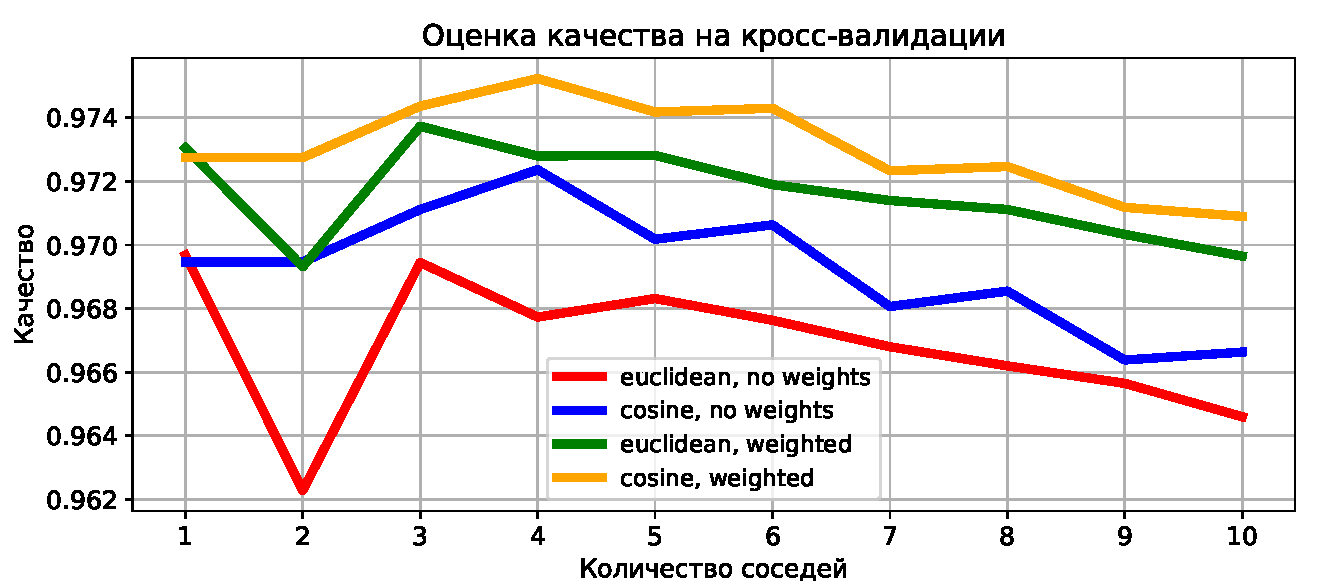
\includegraphics[width=\textwidth]{23_cv_acc.pdf}
    \caption{}
    \label{fig:23_cv_acc}
\end{figure}
По кросс-валидации видно, что косинусная метрика даёт большее качество модели. Использование весов улучшает качество для обеих метрик.

Также по графику ~\autoref{fig:23_cv_acc} видно, что оптимально использование метода 4-х ближайших соседей (чётность не влияет, потому что веса $w \neq 1$)

Напомним, что качество на кросс-валидации усреднялось по 3-м фолдам. Лучшее среднее качество: \textbf{97.52(3)\%},при методе $k=4$ ближайших соседей с весами и косинусной метрикой.

В собственном переборном алгоритме \verb|my_own| эффективно реализован подсчёт расстояний до соседей: один раз строится таблица с расстояними до самого дальнего соседа, потом <<отбрасываются лишние соседи>>.

Также требовалось измерить время поиска $k = 10$ соседей в процессе кросс-валидации. Результат на \autoref{fig:23_cv_time}.

\begin{figure}[h]
\begin{center}
    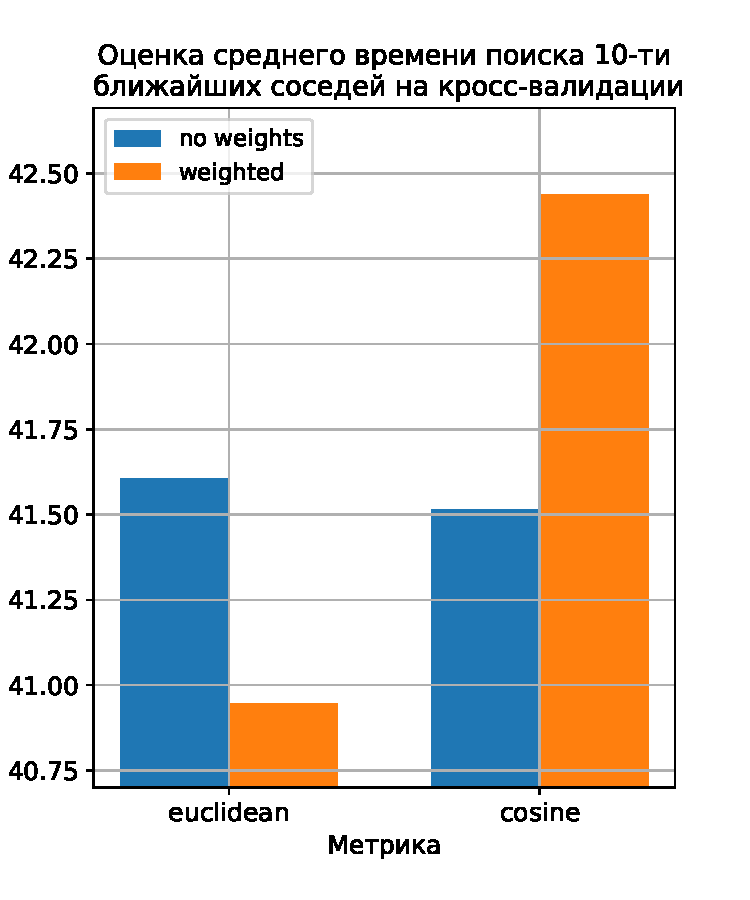
\includegraphics[width=10cm]{23_cv_time.pdf}
    \caption{}
    \label{fig:23_cv_time}
\end{center}
\end{figure}


При подсчёте расстояния по метрике $euclidean$ использовалась формула:
\begin{equation}
    \rho_{\scriptscriptstyle{L_2}}(\mathbf{x},\mathbf{y}) = \Vert{\mathbf{x} - \mathbf{y}}\Vert_2 = \sqrt{\langle\mathbf{x} - \mathbf{y}, \mathbf{x} - \mathbf{y}\rangle} = \sqrt{\Vert{\mathbf{x}}\Vert_2^2 - 2\langle\mathbf{x}, \mathbf{y}\rangle + \Vert{\mathbf{y}}\Vert_2^2}
\end{equation}

При подсчёте расстояния по метрике $cosine$ использовалась формула:
\begin{equation}
    \rho_{\scriptscriptstyle{cos}}(\mathbf{x},\mathbf{y}) = 1-\frac{\langle\mathbf{x}, \mathbf{y}\rangle}
    {\Vert{\mathbf{x}}\Vert \cdot \Vert{\mathbf{y}}\Vert} = 
    1-\left\langle
        \frac{\mathbf{x}}{\Vert{\mathbf{x}}\Vert},
        \frac{\mathbf{y}}{\Vert{\mathbf{y}}\Vert}
    \right\rangle
\end{equation}

\section{Эксперимент №4: качество модели}

В эксперименте №4 требуется оценить качество лучшей модели, сравнить с качеством на кросс-валидации с 3-мя фолдами, сравнить с качеством в Интернете и выяснить, на каких объектах модель ошибается.

На экспериментах №1-3 были подобраны лучшие гиперпараметры и алгоритмы --- взвешенные переборные алгоритмы с метрикой $cosine$ и $k = 4$:~\verb|brute| (самый быстрый) и \verb|my_own|. Обучим модель, соответствующую алгоритму \verb|brute|, на обучающей выборке, получим предсказания на тестовой выборке, проанализируем их.

\begin{itemize} 
        \item Качество на тестовой выборке: \textbf{97.52\%}
        \item Среднее качество на кросс-валидации: \textbf{97.52(3)\%}
\end{itemize} 
Различие незначительное, кросс-валидация сработала хорошо, в ней применялся следующий алгоритм:
сначала датасет MNIST (обучающая выборка) перемешивался, а потом последовательно разбивался на фолды.


Качество лучших алгоритмов на датасете MNIST, согласно рейтингу \cite{topmnist}: \textbf{99.87\%}, результат 2020-го года. В своей статье \cite{byerly2020branching} авторы используют Homogeneous Vector Capsules и свёрточные нейронные сети.


Вернёмся к нашей модели, посмотрим, где она ошибается.
На \autoref{fig:4_conf_mat} изображена матрица ошибок лучшего алгоритма.
\begin{figure}[h]
    \centering
    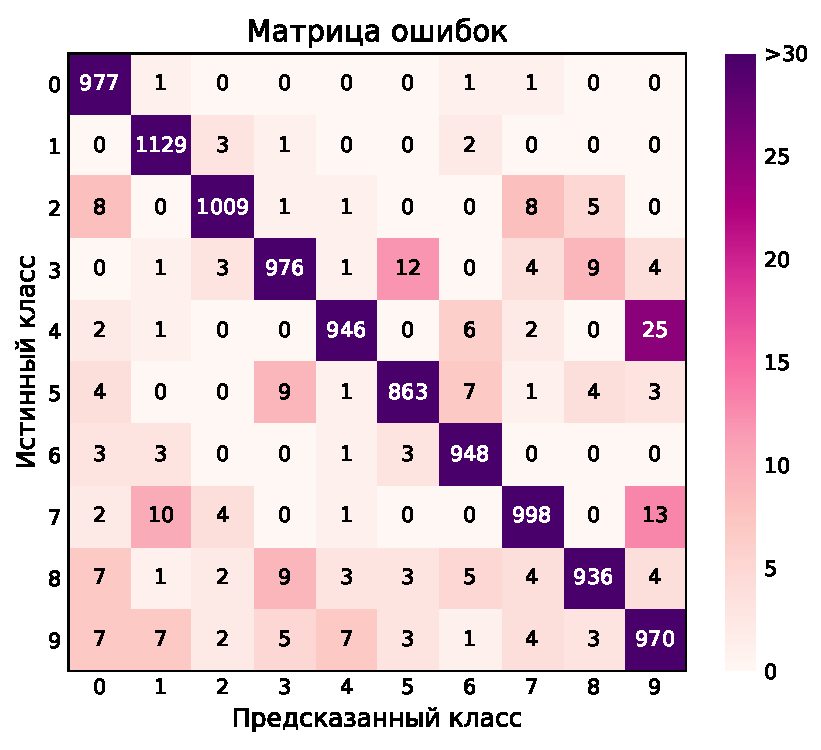
\includegraphics{4_conf_mat}
    \caption{}
    \label{fig:4_conf_mat}
\end{figure}

Визуальный анализ матрицы ошибок (\autoref{fig:4_conf_mat}) показал, что:
\begin{itemize}
    \item Цифры \textit{\textbf{0}} и \textit{\textbf{1}} классифицируются лучше всего (меньше всего ошибок). Видимо, это из-за небольшого количества <<простых линий>> в их символах.
    \item Цифры \textit{\textbf{8}} и \textit{\textbf{9}} классифицируются хуже всего (больше всего ошибок). Видимо, это из-за <<переплетений линий>> в их символах.
    \item Алгоритм нередко распознаёт истинную \textbf{\textit{3}} как \textbf{\textit{5}} (12 раз) и наоборот (9 раз) (иногда ошибки симметричны, но в основном --- нет)
    \item Самые частые ошибки:
    \begin{enumerate}
        \item (25 раз) Распознавание истинной \textit{\textbf{4}} как \textit{\textbf{9}}
        \item (13 раз) Распознавание истинной \textit{\textbf{7}} как \textit{\textbf{9}}
        \item (12 раз) Распознавание истинной \textit{\textbf{3}} как \textit{\textbf{5}}
        \item (10 раз) Распознавание истинной \textit{\textbf{7}} как \textit{\textbf{1}}
    \end{enumerate}
\end{itemize}

Далее на \autoref{fig:4_mistakes_bold},~\autoref{fig:4_mistakes_rotated},~\autoref{fig:4_mistakes_similar},~\autoref{fig:4_mistakes_strange} визуализированы некоторые группы\\
ошибочно классифицированных объектов с общими чертами.
\begin{figure}[!h]
    \centering
    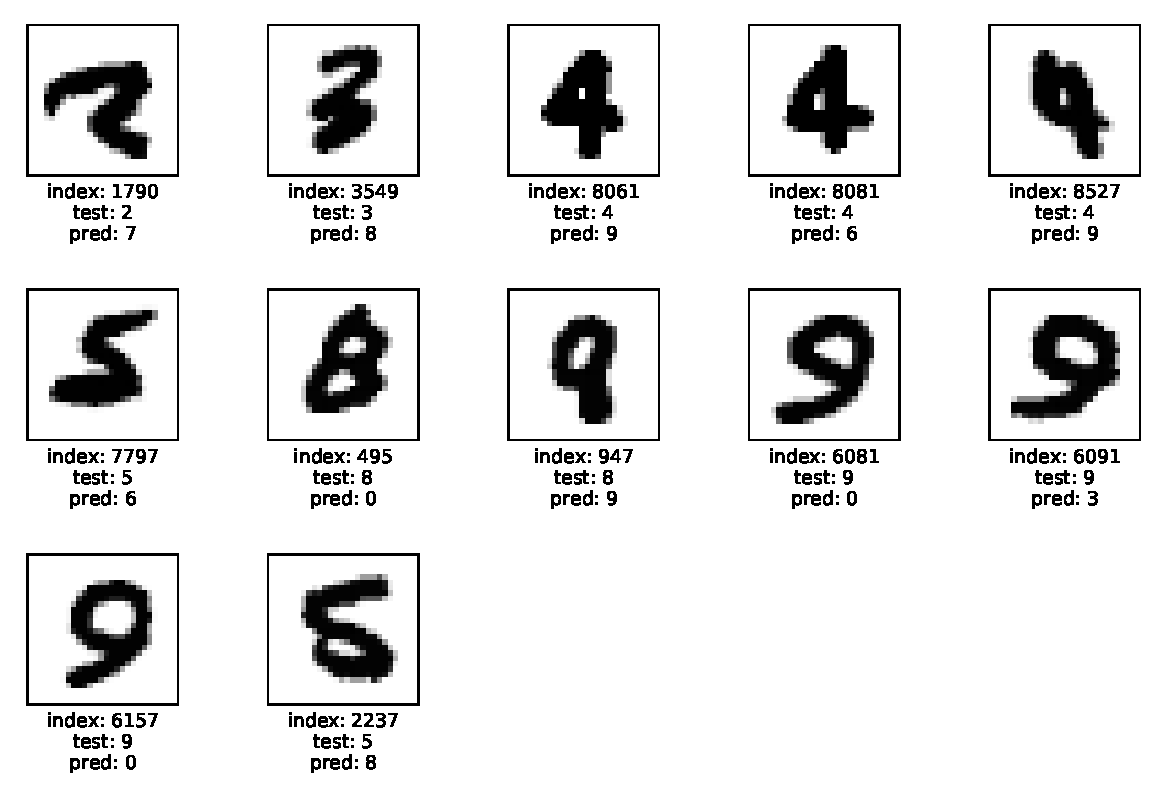
\includegraphics[width=\textwidth]{4_mistakes_bold}
    \caption{Группа 1: слишком жирное написание}
    \label{fig:4_mistakes_bold}
\end{figure}
\begin{figure}[!h]
    \centering
    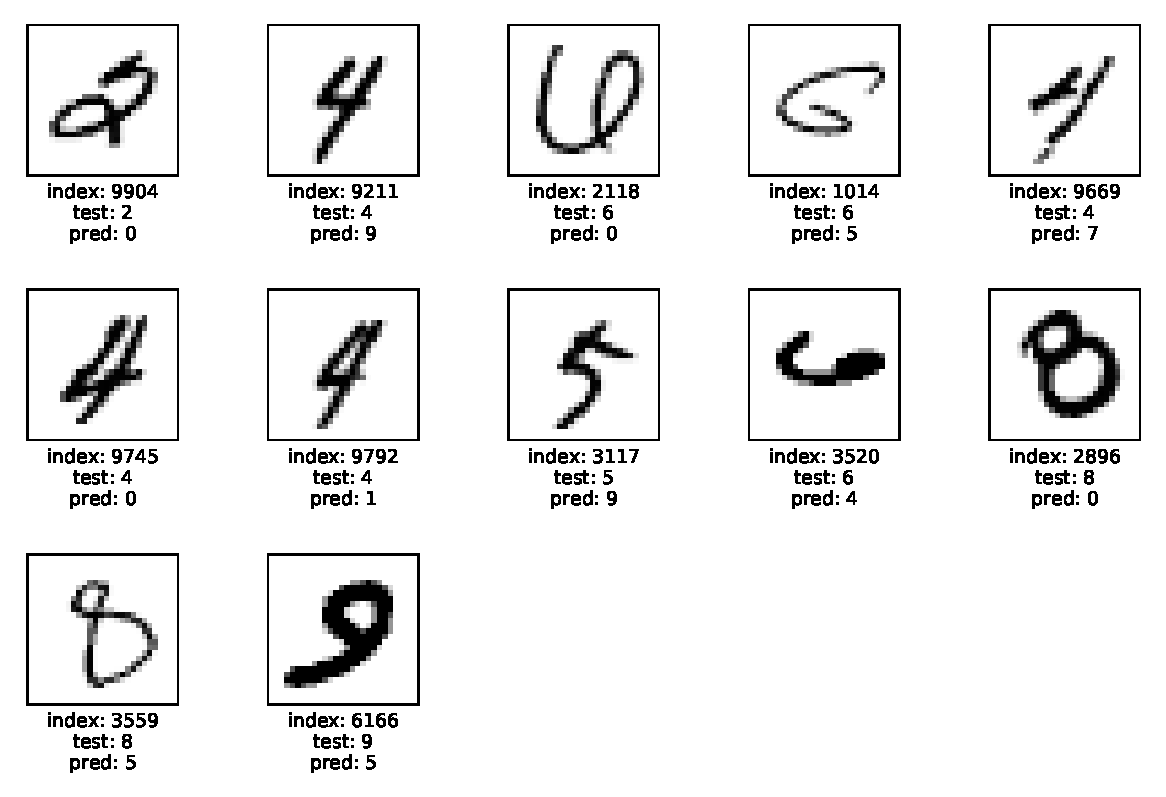
\includegraphics[width=\textwidth]{4_mistakes_rotated}
    \caption{Группа 2: повёрнутые цифры}
    \label{fig:4_mistakes_rotated}
\end{figure}
\begin{figure}[!h]
    \centering
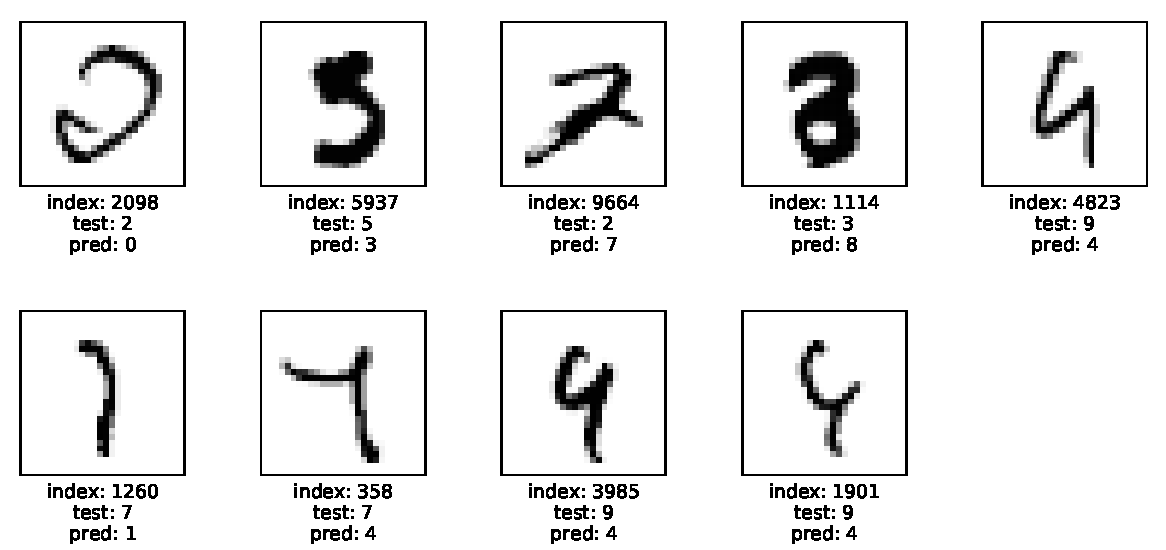
\includegraphics[width=\textwidth]{4_mistakes_similar}
    \caption{Группа 3: цифры, очень похожие на другие (неоднозначная классификация)}
    \label{fig:4_mistakes_similar}
\end{figure}
\begin{figure}[!h]
    \centering
    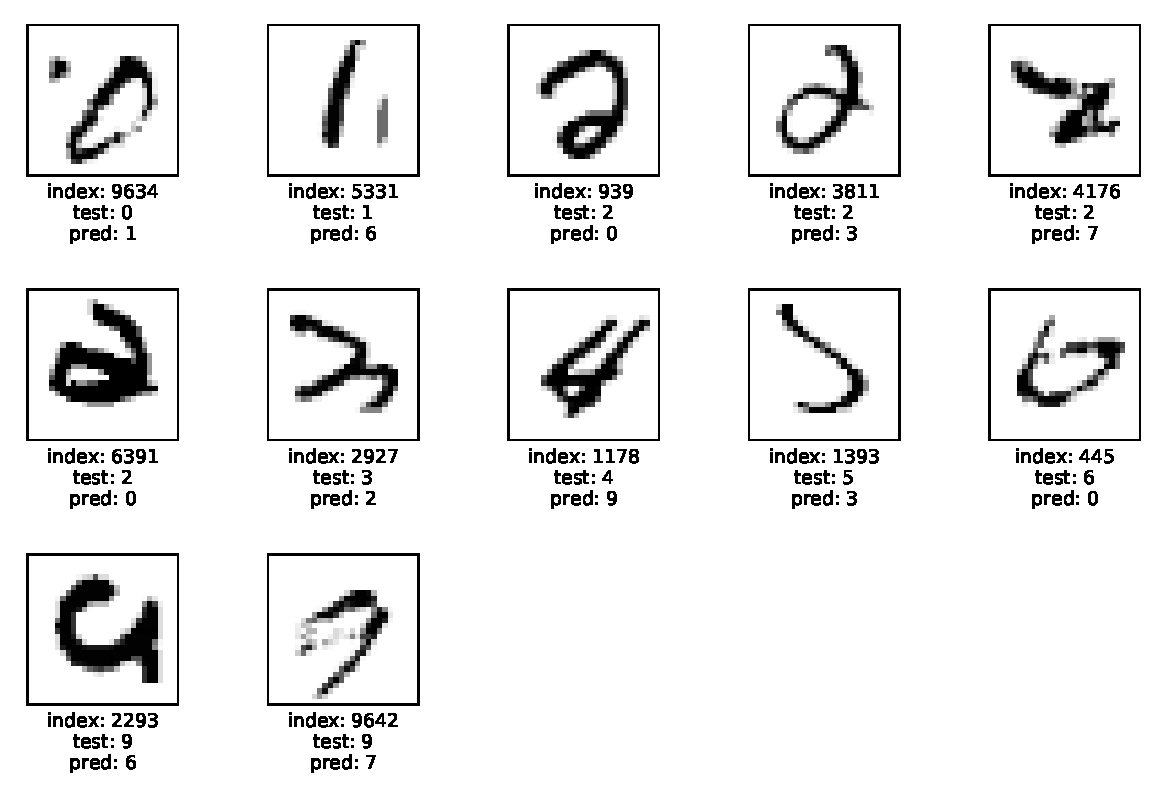
\includegraphics[width=\textwidth]{4_mistakes_strange}
    \caption{Группа 4: трудно классифицируемые символы}
    \label{fig:4_mistakes_strange}
\end{figure}

\section{\mbox{Эксперимент №5: аугментация обучающей выборки}}

В эксперименте №5 требуется размножить (аугментировать) обучающую выборку с помощью следующих преобразований:
\begin{itemize}
    \item Поворот изображений на: $\pm5\degree$, $\pm10\degree$, $\pm15\degree$
    \item Сдвиг изображений на: $\pm1$px, $\pm2$px, $\pm3$px (по каждой из двух размерностей)
    \item Применение к изображениям фильтра Гаусса с дисперсией: $0.5$, $1.0$, $1.5$
\end{itemize}

После чего требуется определить качество модели на различных преобразованиях и влияние этих преобразований.

Выполним кросс-валидацию на лучшем (то есть метрика $cosine$, алгоритм с весами) алгоритме, \verb|brute|-алгоритме. Выясним оптимальное число $k$ ближайших соседей при разных трансформациях.
Выборка преобразуется таким образом: к исходной выборке прибавляется трансформированная. Например, в случае сдвига аугментированная обучающая выборка будет состоять из исходной выборки и двух трансформированных (преобразование по одной из осей и в противоположном направлении, например +1px и -1px по горизонтали). То есть в этом примере аугментированная выборка будет в три раза больше исходной обучающей выборки.

Далее на \autoref{fig:5_aug_cv_acc} приведены результаты кросс-валидации. Для сравнения на графике пунктиром приводится график этого же лучшего алгоритма, с теми же гиперпараметрами, но без аугментации.

\begin{figure}[!h]
    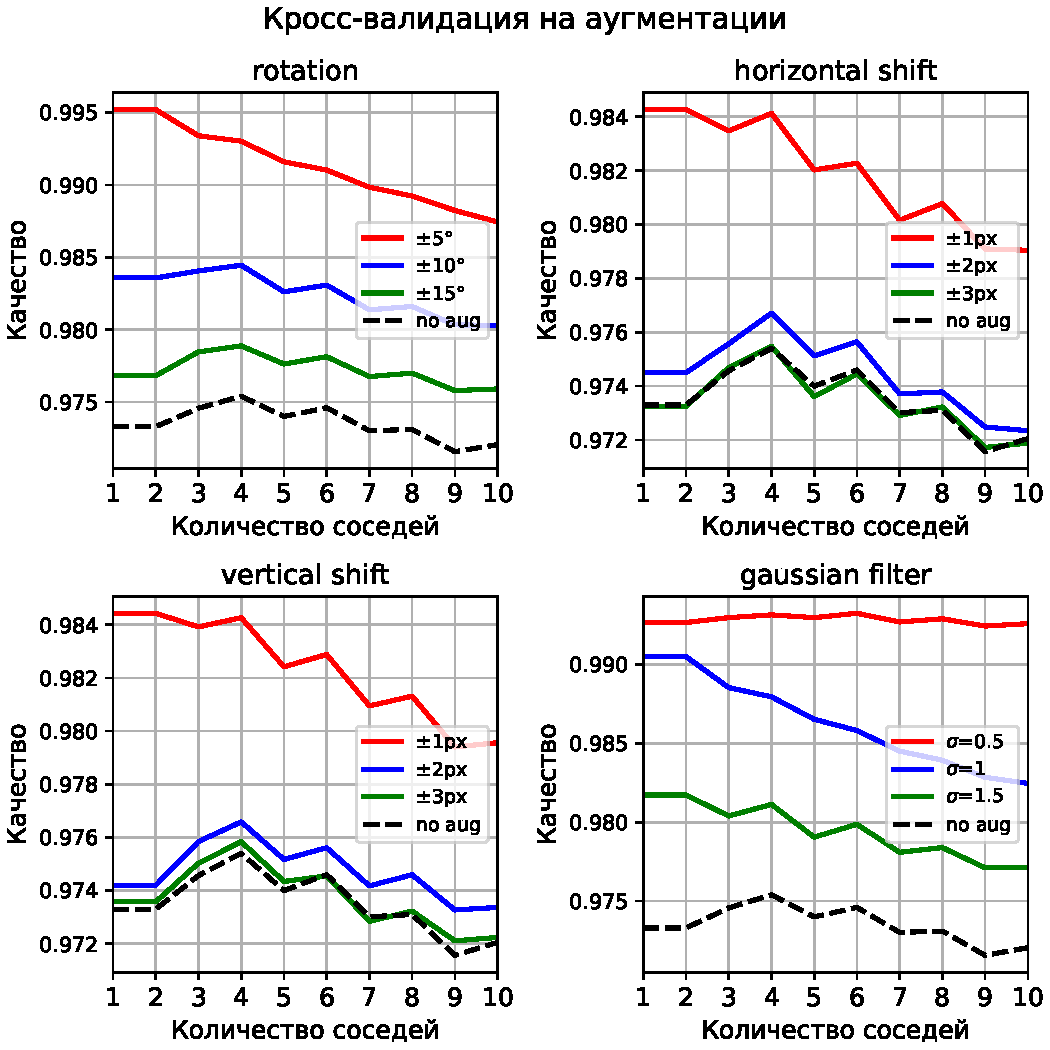
\includegraphics[width=\textwidth]{5_aug_cv_acc}
    \caption{}
    \label{fig:5_aug_cv_acc}
\end{figure}

Исходя из графиков, лучшие параметры трансформаций:
\begin{itemize}
    \item Поворот изображений на: $\pm5\degree$
    \item Сдвиг изображений на: $\pm1$px (по каждой из двух размерностей)
    \item Применение к изображениям фильтра Гаусса с дисперсией: $0.5$
\end{itemize}
Далее в этом эксперименте мы объединим сдвиги по разным осям (при трансформации сдвигом, выборка увеличится в 5 раз: исходная выборка + по 2 трансформированные выборки по каждой из осей)

Также, исходя из графиков, оптимальный параметр $k$:
\begin{itemize}
    \item При повороте: $k = 2$
    \item При сдвиге: $k = 4$
    \item При размытии: $k = 6$
\end{itemize}

Руководствуясь этими гиперпараметрами, сделаем предсказания на всех видах аугментированных по лучшим параметрам трансформаций выборках. То есть предсказания на выборках, аугментированных с помощью поворота на $\pm5\degree$, сдвига на $\pm1$px, размытия фильтром Гаусса с дисперсией $0.5$, и на комбинациях этих аугментированных обучающих выборок. Назовём эти варианты аугментации и их комбинации как: \textbf{rotation}, \textbf{shift}, \textbf{gauss}, \textbf{rotation+shift}, \textbf{rotation+gauss}, \textbf{shift+gauss}, \textbf{rotation+shift+gauss}. Вариант работы алгоритма без аугментации обучающей выборки (нужно для сравнения) назовём \textbf{no\_aug}.

\break

Далее на \autoref{fig:5_aug_conf_mat_1} и на \autoref{fig:5_aug_conf_mat_2} представлены матрицы ошибок для всех описанных случаев. Видно, как разные аугментации уменьшают число различных ошибок в матрице.
\begin{figure}[!h]
    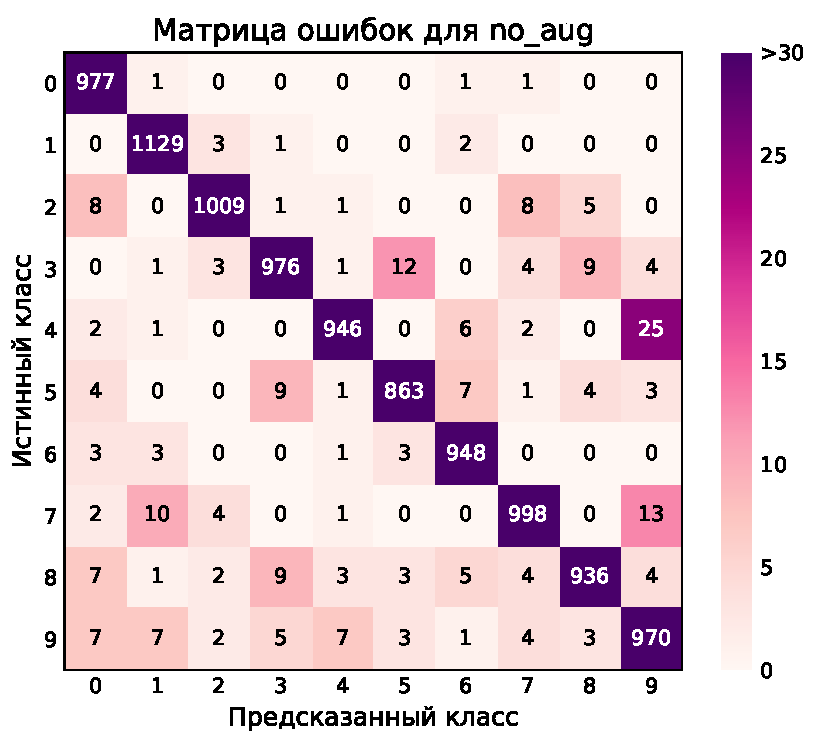
\includegraphics[scale=0.6]{5_aug_conf_mat_no_aug.pdf}
    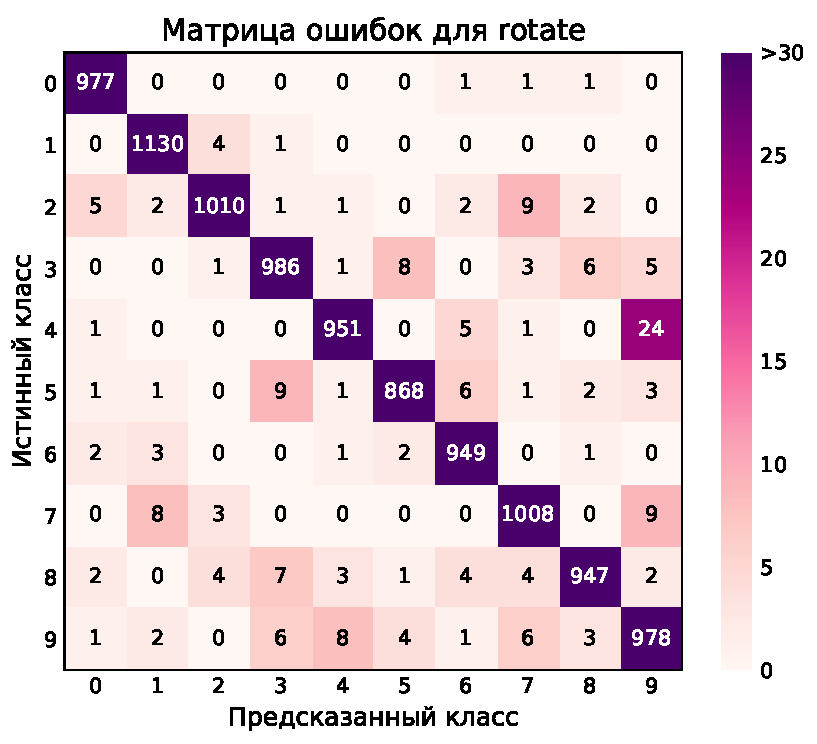
\includegraphics[scale=0.6]{5_aug_conf_mat_rotate.pdf}
    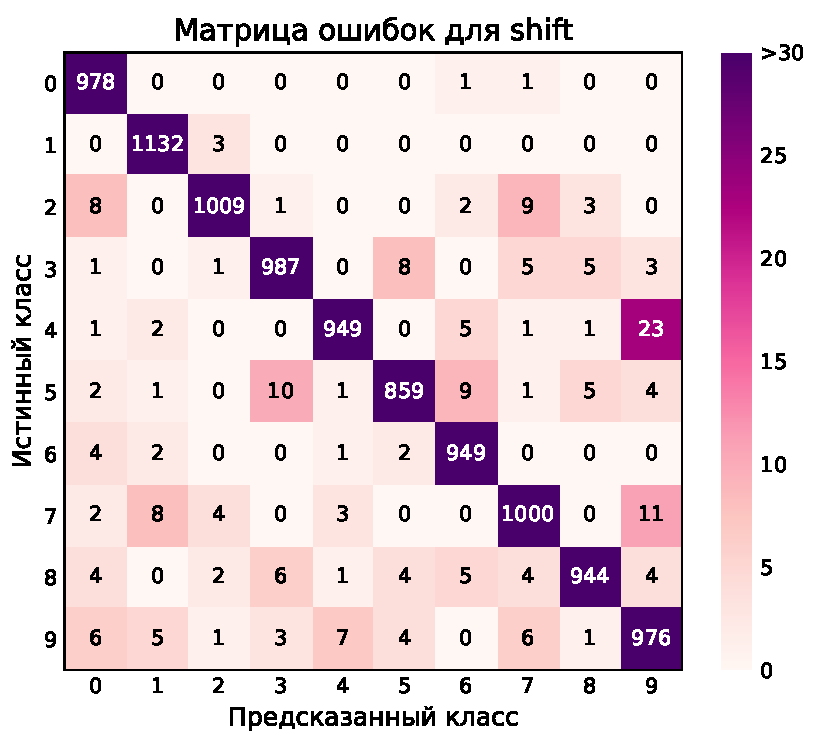
\includegraphics[scale=0.6]{5_aug_conf_mat_shift.pdf}
    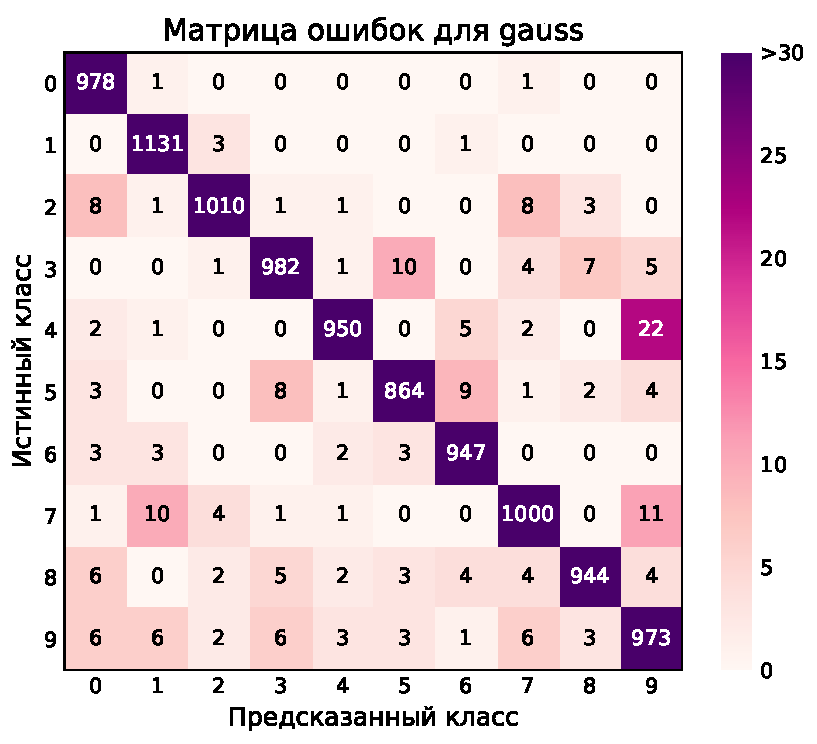
\includegraphics[scale=0.6]{5_aug_conf_mat_gauss.pdf}
    \caption{Матрицы ошибок на аугментированных выборках}
    \label{fig:5_aug_conf_mat_1}
\end{figure}
\begin{figure}[!h]
    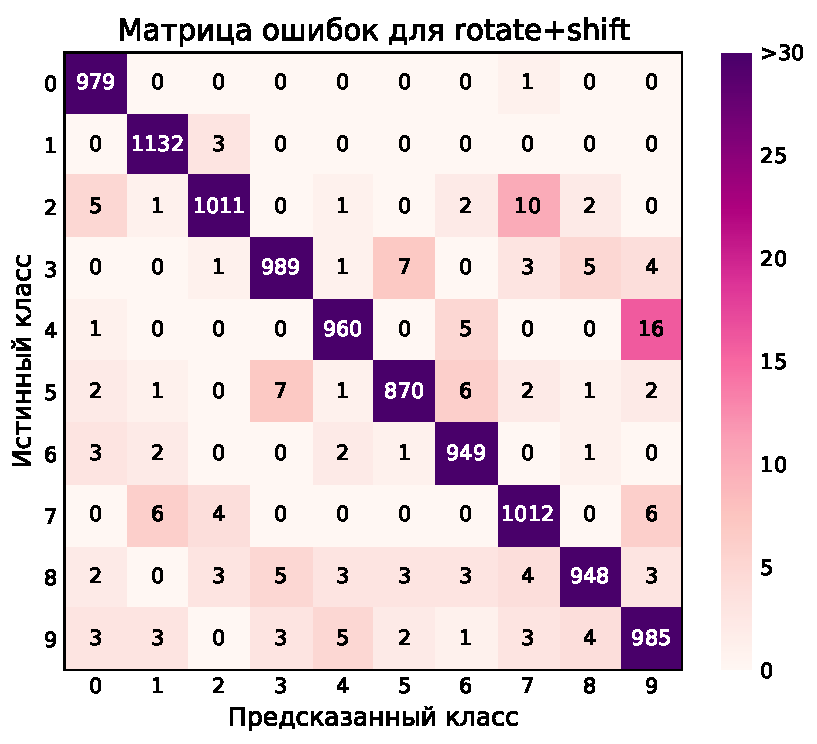
\includegraphics[scale=0.6]{5_aug_conf_mat_rotate+shift.pdf}
    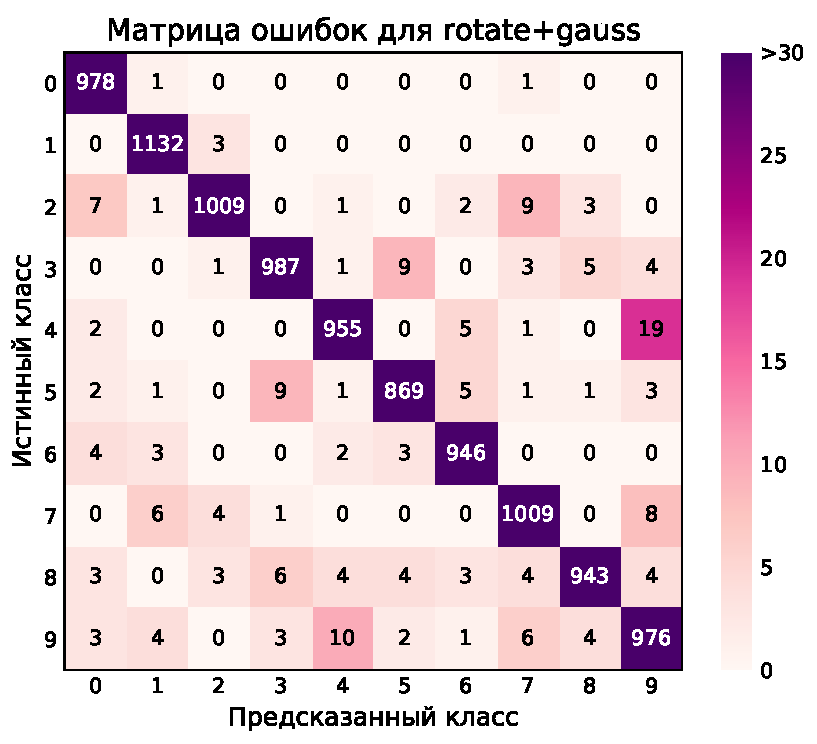
\includegraphics[scale=0.6]{5_aug_conf_mat_rotate+gauss.pdf}
    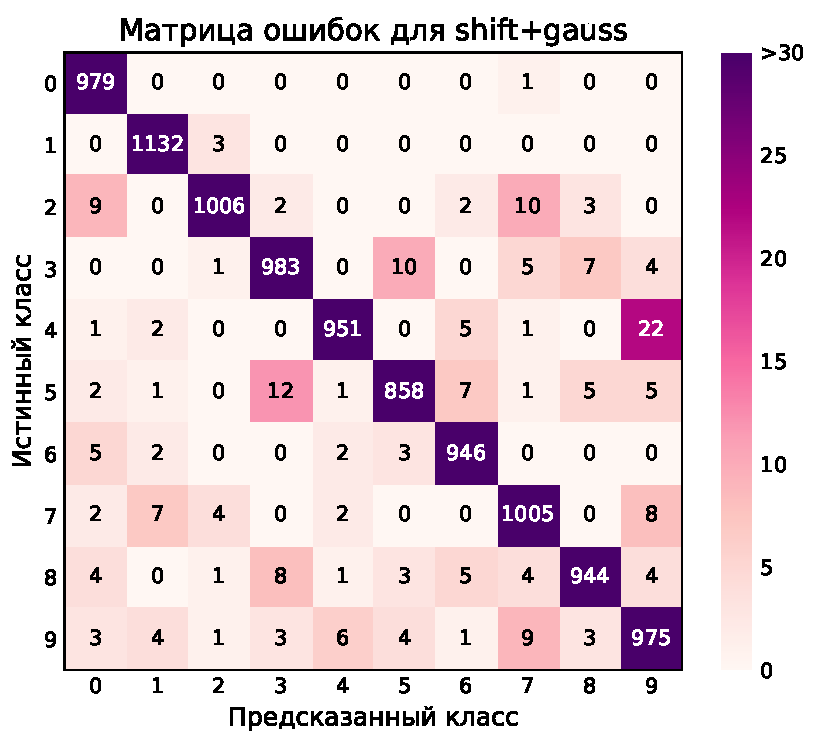
\includegraphics[scale=0.6]{5_aug_conf_mat_shift+gauss.pdf}
    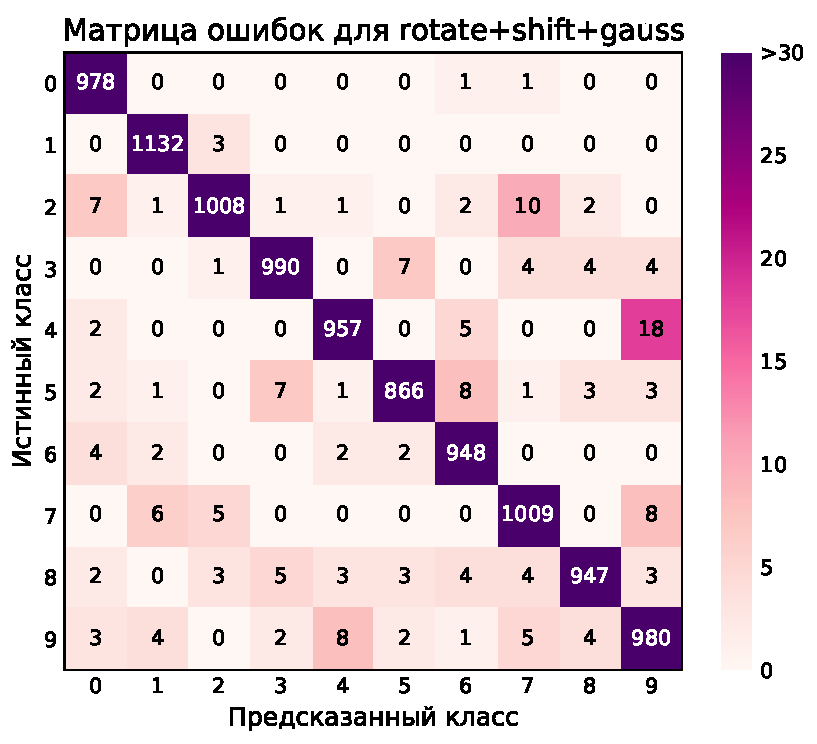
\includegraphics[scale=0.6]{5_aug_conf_mat_rotate+shift+gauss.pdf}
    \caption{Матрицы ошибок на комбинациях аугментированных выборок}
    \label{fig:5_aug_conf_mat_2}
\end{figure}

Преобразования поворота исправляли ошибки классификации на повёрнутых цифрах, преобразования смещения --- на нецентрированных цифрах, а преобразование размытия фильтром Гаусса --- на жирно написанных цифрах.

По матрицам ошибок явно видно, как уменьшаются ошибки на различных преобразованиях.
Две самые распространённые ошибки: распознавания истинной \textit{\textbf{4}} как \textit{\textbf{9}} и распознавания истинной \textit{\textbf{7}} как \textit{\textbf{9}} --- эти ошибки были уменьшены на комбинациях, в которых есть поворот: \textbf{rotate+shift}, \textbf{rotate+shift+gauss}, \textbf{rotate+shift}, \textbf{rotate+gauss}. Также примерно все методы уменьшили распознавание истинного \textit{\textbf{0}} как другой цифры. А вот количество ошибок распознавания истинной \textit{\textbf{2}} как \textit{\textbf{7}} увеличилось или осталось прежним.

На \autoref{tab:5_acc_tab} приведён итог эксперимента №5. Лучшее качество \textbf{97.35\%} достигается при сочетании поворотов на $\pm5\degree$ и сдвигов на $\pm1$px (по обеим осям).
\newpage
\begin{center}
\begin{table}[!h]
    \begin{center}
    \begin{tabular}[!h]{ | l | l | }
    \hline
    Аугментированная выборка & Качество (\%)\\ \hline
    no\_aug & 97.52\\
    rotate & 98.04\\
    shift & 97.83\\
    gauss & 97.78(9)\\
    rotate+shift & 98.35\\
    rotate+gauss & 98.04\\
    shift+gauss & 97.78(9)\\
    rotate+shift+gauss & 98.15\\
    \hline
    \end{tabular}
    \caption{Качество модели на аугментированных обучающих выборках при всех типах преобразований и при всех комбинациях. Лучшее качество: \textbf{98.35\%}.}
    \label{tab:5_acc_tab}
    \end{center}
\end{table}
\end{center}

Вывод из эксперимента №5: с помощью различных аугментаций на обучающей выборке можно исправлять качественно разные ошибки алгоритма, корректировать его.

% \newpage
\section{Эксперимент №6: аугментация тестовой выборки}

В эксперименте №6 требуется размножить объекты тестовой выборки, то есть сделать аугментацию тестовой выборки, а для её преобразований использовать те же, что и в эксперименте~№5:
\begin{itemize}
    \item Поворот изображений на: $\pm5\degree$, $\pm10\degree$, $\pm15\degree$
    \item Сдвиг изображений на: $\pm1$px, $\pm2$px, $\pm3$px (по каждой из двух размерностей)
    \item Применение к изображениям фильтра Гаусса с дисперсией: $0.5$, $1.0$, $1.5$
\end{itemize}

После чего требуется определить качество модели на различных преобразованиях и влияние этих преобразований, аналогично эксперименту №5, но только аугментация не на обучающей, а на тестовой выборке. Будем искать расстояния при различных преобразованиях тестовой выборки по стратегии наименьшего расстояния, что согласуется с гипотезой компактности \cite{compact} и идей метода $k$ ближайших соседей. То есть среди всех аугментированных тестовых выборок выбирается наименьшее расстояние для этого объекта.

Выберем параметры трансформации по той же схеме, что и в эксперименте~№5.

Выполним кросс-валидацию на лучшем (то есть метрика $cosine$, алгоритм с весами) алгоритме, \verb|my_own|-алгоритме. Выясним оптимальное число $k$ ближайших соседей при разных трансформациях.

Далее на \autoref{fig:6_aug_cv_acc} приведены результаты кросс-валидации. Для сравнения на графике пунктиром приводится график этого же лучшего алгоритма, с теми же гиперпараметрами, но без аугментации.

\begin{figure}[!h]
    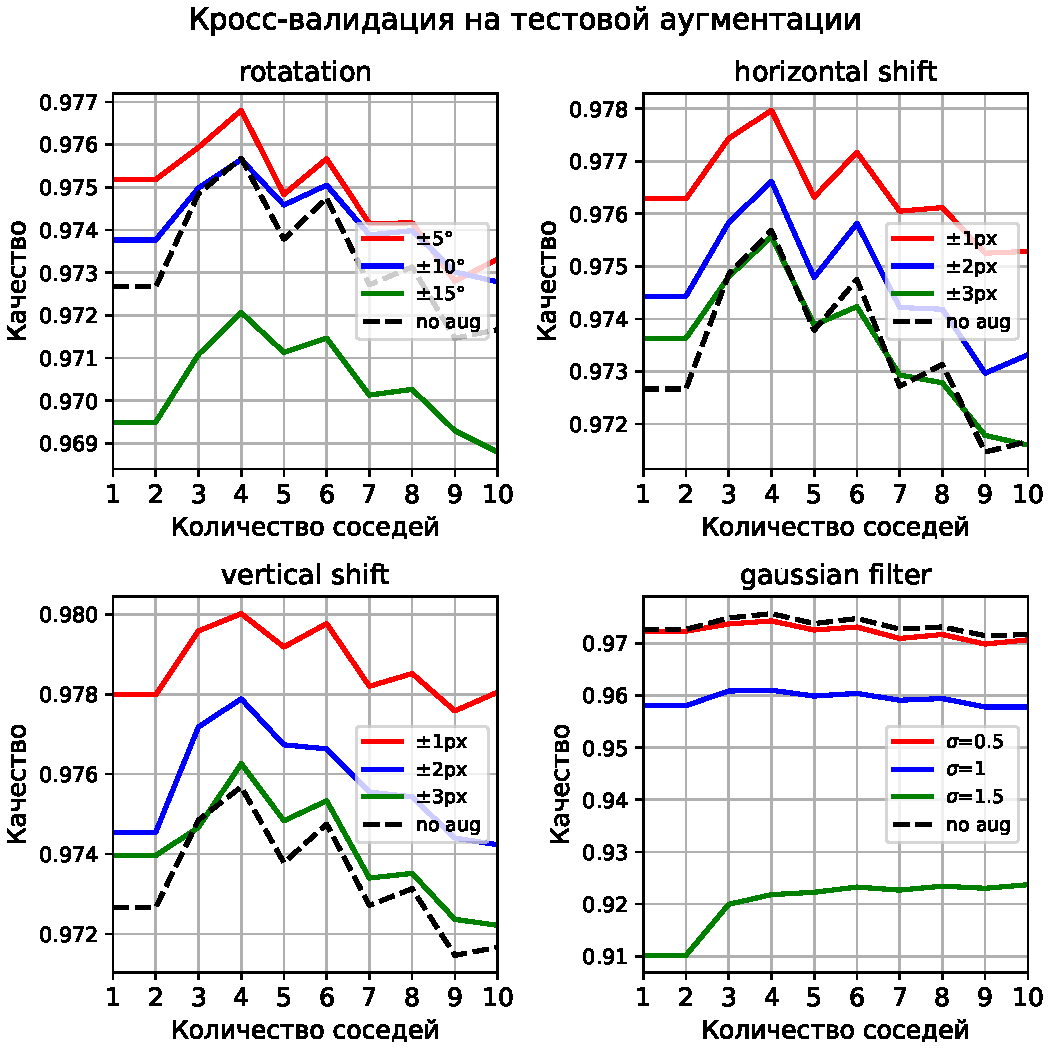
\includegraphics[width=\textwidth]{6_aug_cv_acc}
    \caption{}
    \label{fig:6_aug_cv_acc}
\end{figure}

Исходя из графиков, лучшие параметры трансформаций остались теми же, только фильтр Гаусса в этот раз ухудшал качество, поэтому для простоты оставим его прежним, с дисперсией $0.5$:
\begin{itemize}
    \item Поворот изображений на: $\pm5\degree$
    \item Сдвиг изображений на: $\pm1$px (по каждой из двух размерностей)
    \item Применение к изображениям фильтра Гаусса с дисперсией: $0.5$
\end{itemize}
Объединим сдвиги по разным осям.

Далее, как видно по графикам, оптимальный параметр $k$ изменился по сравнению с предыдущим экспериментом. Теперь это везде $k = 4$:
\begin{itemize}
    \item При повороте: $k = 4$
    \item При сдвиге: $k = 4$
    \item При размытии: $k = 4$
\end{itemize}

Аналогично предыдущему эксперименту, руководствуясь подобранными гиперпараметрами, сделаем предсказания на всех видах аугментированных по лучшим параметрам трансформаций выборках.

\break

Далее на \autoref{fig:6_aug_conf_mat_1} и на \autoref{fig:6_aug_conf_mat_2} представлены матрицы ошибок для всех описанных случаев.
\begin{figure}[!h]
    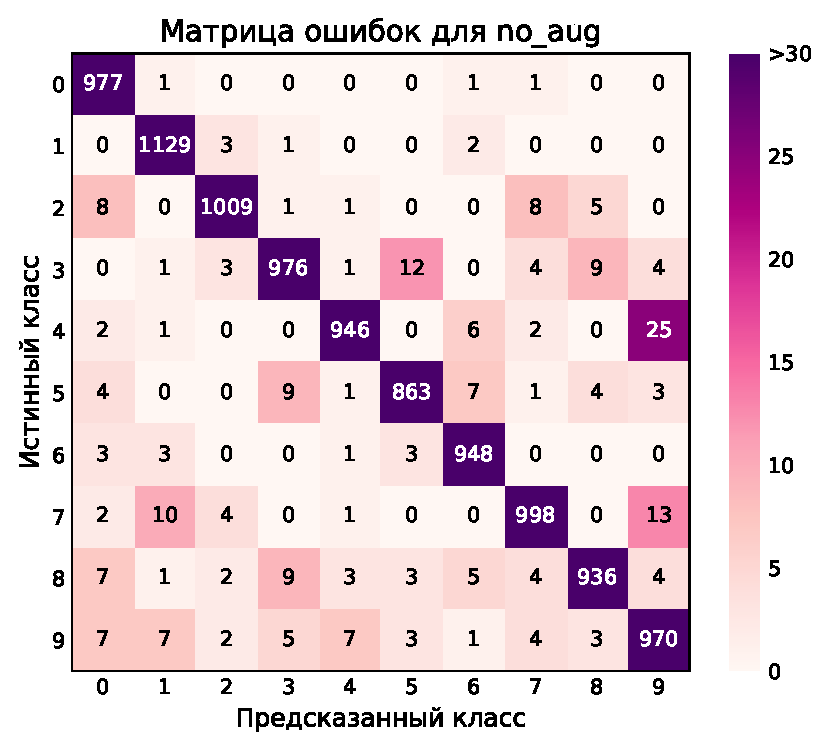
\includegraphics[scale=0.6]{6_aug_conf_mat_no_aug.pdf}
    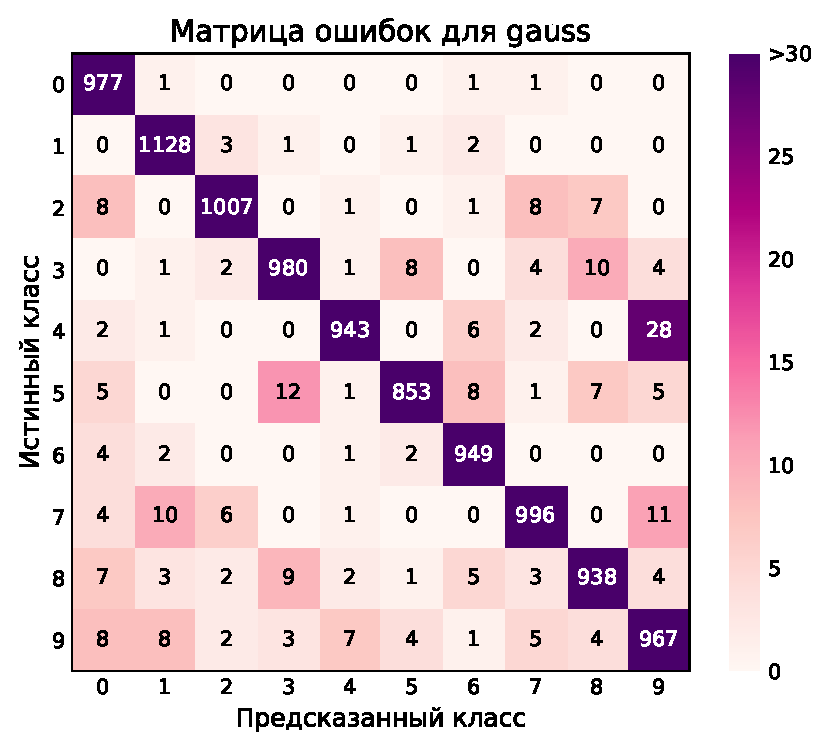
\includegraphics[scale=0.6]{6_aug_conf_mat_gauss.pdf}
    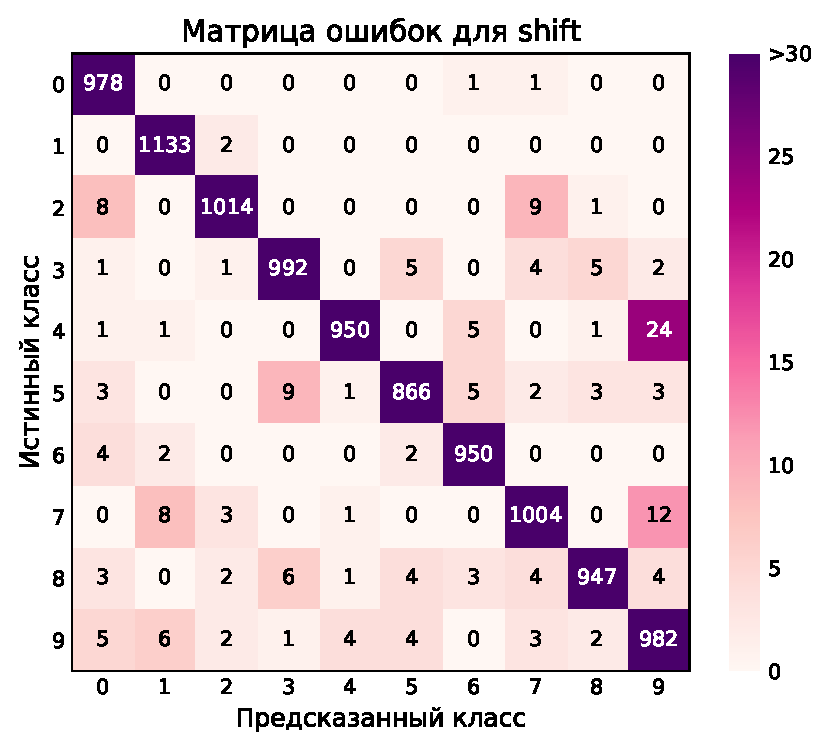
\includegraphics[scale=0.6]{6_aug_conf_mat_shift.pdf}
    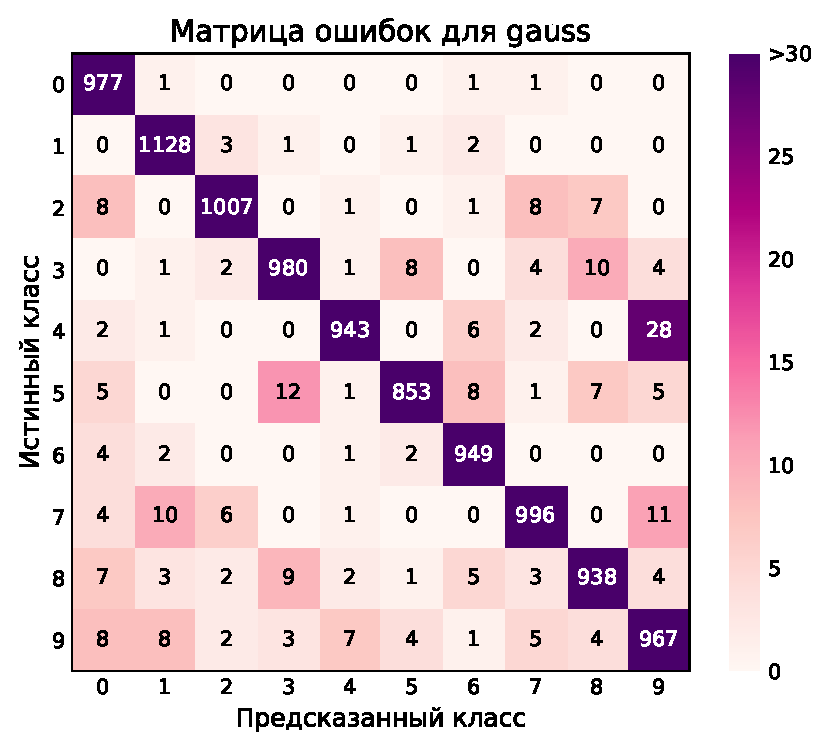
\includegraphics[scale=0.6]{6_aug_conf_mat_gauss.pdf}
    \caption{Матрицы ошибок на аугментированных тестовых выборках}
    \label{fig:6_aug_conf_mat_1}
\end{figure} 
\begin{figure}[!h]
    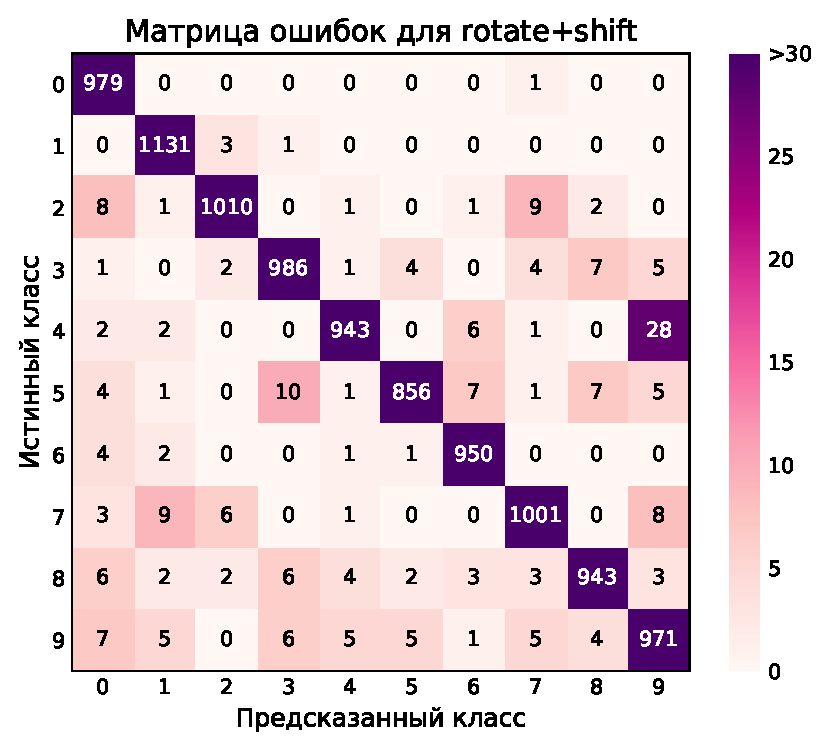
\includegraphics[scale=0.6]{6_aug_conf_mat_rotate+shift.pdf}
    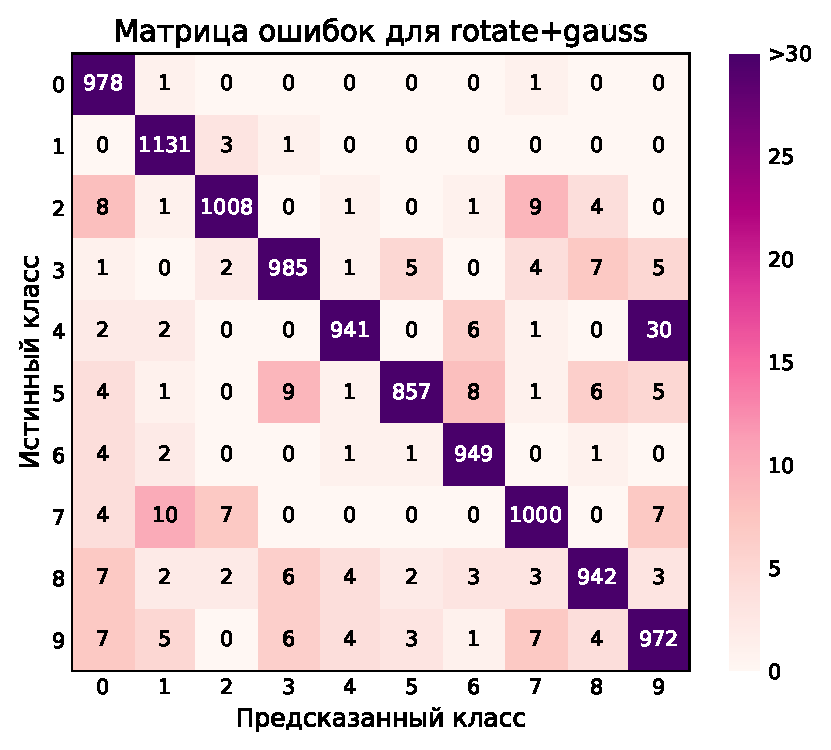
\includegraphics[scale=0.6]{6_aug_conf_mat_rotate+gauss.pdf}
    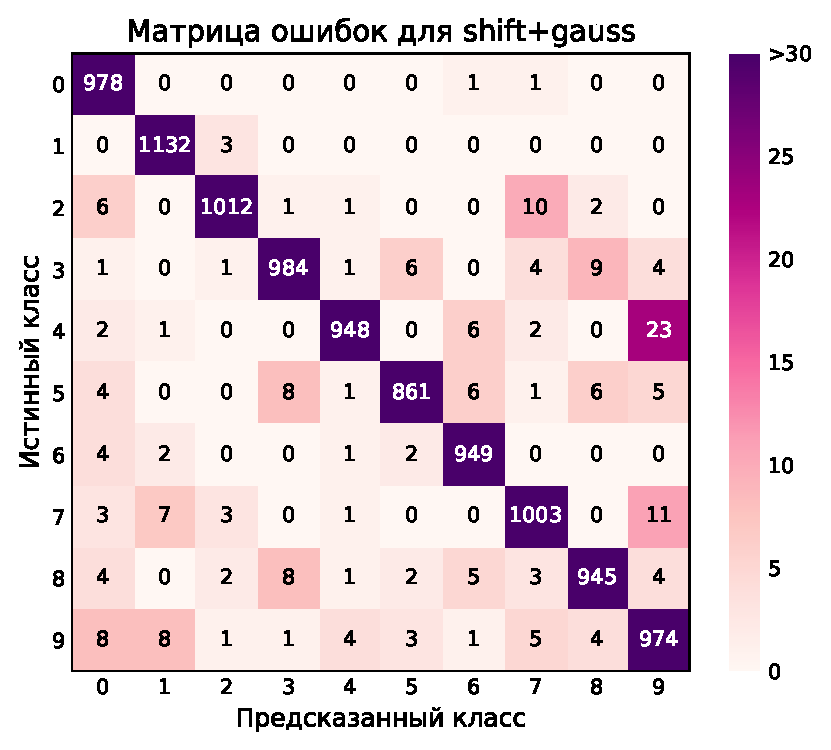
\includegraphics[scale=0.6]{6_aug_conf_mat_shift+gauss.pdf}
    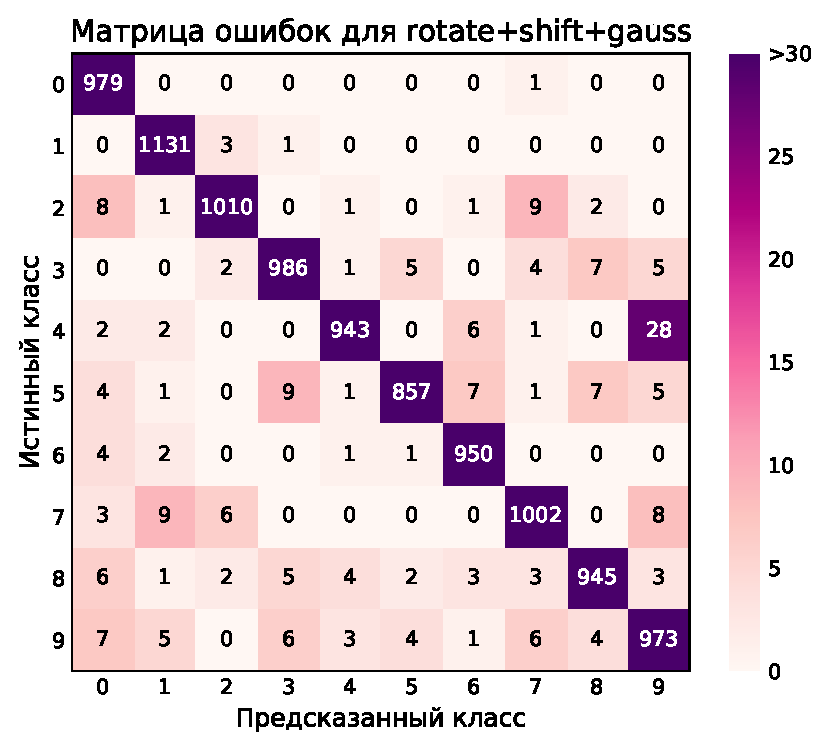
\includegraphics[scale=0.6]{6_aug_conf_mat_rotate+shift+gauss.pdf}
    \caption{Матрицы ошибок на комбинациях аугментированных тестовых выборок}
    \label{fig:6_aug_conf_mat_2}
\end{figure}

Как и в прошлом эксперименте, преобразования поворота исправляли ошибки классификации на повёрнутых цифрах. Фильтр Гаусса справился с хуже, чем в эксперименте №5. В целом видно, что качество стало хуже в сравнении с предыдущим экспериментом.

По матрицам ошибок видно, что фильтр Гаусса ухудшает качество модели, в сравнении с экспериментом №5.
Если в аугментации обучающей выборки фильтр Гаусса, <<сглаживая>> шум, обучает алгоритм лучше, то в аугментации тестовой выборки фильтр Гаусса <<затирает>> нужную для классификации информацию, внося в классификацию больше <<неопределённости>>. Повороты и сдвиги вносят примерно равный полезный вклад, что в этом эксперименте, что в эксперименте №5. Но в случае аугментации обучающей выборки лучше работают повороты, а в случае аугментации тестовой выборки --- сдвиги.

На \autoref{tab:6_acc_tab} приведён итог эксперимента №6. Лучшее качество \textbf{97.35\%} достигается сдвигах на $\pm1$px (по обеим осям).
\newpage
\begin{center}
\begin{table}[!h]
    \begin{center}
    \begin{tabular}[!h]{ | l | l | }
    \hline
    Аугментированная выборка & Качество (\%)\\ \hline
    no\_aug & 97.52\\
    rotate & 97.6\\
    shift & 98.16\\
    gauss & 97.38\\
    rotate+shift & 97.7\\
    rotate+gauss & 97.63\\
    shift+gauss & 97.86\\
    rotate+shift+gauss & 97.76\\
    \hline
    \end{tabular}
    \caption{Качество модели на аугментированных тестовых выборках при всех типах преобразований и при всех комбинациях. Лучшее качество: \textbf{98.16\%}.}
    \label{tab:6_acc_tab}
    \end{center}
\end{table}
\end{center}

\section{Заключение}
Итого на примере датасета MNIST был проведен ряд экспериментов с методом классификации $kNN$.
В данном примере лучшие гиперпараметры оказались такими: метрика --- косинусная, веса в алгоритме --- да, $k = 4$. При этом, для нашей задачи эффективны (по скорости работы) переборные алгоритмы $kNN$, а не деревья. Сравнивались два различных метода аугментации выборок: обучающей и тестовой. Оба подхода имеют свои преимущества и недостатки, но лучший результат показала аугментация обучающей выборки: на ней лучшее качество \textbf{98.35\%} достигается при сочетании поворотов и сдвигов. Итоговое качество~--- \textbf{98.35\%}.

\selectlanguage{english}
\printbibliography
\end{document}